\documentclass{article}

\usepackage{arxiv}

\usepackage[utf8]{inputenc} % allow utf-8 input
\usepackage[T1]{fontenc}    % use 8-bit T1 fonts
\usepackage{lmodern}        % https://github.com/rstudio/rticles/issues/343
\usepackage{hyperref}       % hyperlinks
\usepackage{url}            % simple URL typesetting
\usepackage{booktabs}       % professional-quality tables
\usepackage{amsfonts}       % blackboard math symbols
\usepackage{nicefrac}       % compact symbols for 1/2, etc.
\usepackage{microtype}      % microtypography
\usepackage{graphicx}

\title{To Batch or Not to Batch: Test-Ordering Variability in the ED}

\author{
    Jacob Jameson
   \\
    Interfaculty Initiative in Health Policy \\
    Harvard University \\
  Cambridge, MA \\
  \texttt{} \\
   \And
    Soroush Saghafian
   \\
    Harvard Kennedy School of Government \\
    Harvard University \\
  Cambridge, MA \\
  \texttt{} \\
   \And
    Robert Huckman
   \\
    Harvard Business School \\
    Harvard University \\
  Boston, MA \\
  \texttt{} \\
   \And
    Nicole Hodgson
   \\
    Emergency Department \\
    Mayo Clinic \\
  Phoenix, AZ \\
  \texttt{} \\
  }


% tightlist command for lists without linebreak
\providecommand{\tightlist}{%
  \setlength{\itemsep}{0pt}\setlength{\parskip}{0pt}}


% Pandoc citation processing
\newlength{\cslhangindent}
\setlength{\cslhangindent}{1.5em}
\newlength{\csllabelwidth}
\setlength{\csllabelwidth}{3em}
\newlength{\cslentryspacingunit} % times entry-spacing
\setlength{\cslentryspacingunit}{\parskip}
% for Pandoc 2.8 to 2.10.1
\newenvironment{cslreferences}%
  {}%
  {\par}
% For Pandoc 2.11+
\newenvironment{CSLReferences}[2] % #1 hanging-ident, #2 entry spacing
 {% don't indent paragraphs
  \setlength{\parindent}{0pt}
  % turn on hanging indent if param 1 is 1
  \ifodd #1
  \let\oldpar\par
  \def\par{\hangindent=\cslhangindent\oldpar}
  \fi
  % set entry spacing
  \setlength{\parskip}{#2\cslentryspacingunit}
 }%
 {}
\usepackage{calc}
\newcommand{\CSLBlock}[1]{#1\hfill\break}
\newcommand{\CSLLeftMargin}[1]{\parbox[t]{\csllabelwidth}{#1}}
\newcommand{\CSLRightInline}[1]{\parbox[t]{\linewidth - \csllabelwidth}{#1}\break}
\newcommand{\CSLIndent}[1]{\hspace{\cslhangindent}#1}

\usepackage{booktabs}
\usepackage{tabularx}
\usepackage{graphicx}
\usepackage{tikz}
\usepackage{siunitx}
\usepackage{tablefootnote}
\usepackage{longtable}
\usepackage{threeparttable}
\usepackage{natbib}
\usepackage{caption}
\usepackage{adjustbox}
\usepackage{multirow}
\begin{document}
\maketitle


\begin{abstract}

\end{abstract}


\hypertarget{introduction}{%
\section{Introduction}\label{introduction}}

Healthcare delivery, particularly in the emergency department (ED), is a
delicate balance that involves ensuring optimal patient outcomes while
optimizing resource utilization. Achieving these twin goals requires
timely and accurate diagnosis, which in turn enables prompt and
appropriate treatment, consequently improving patient prognosis and
reducing the likelihood of adverse events. Furthermore, efficient
patient discharge from the ED can help alleviate overcrowding, a severe
issue with potential consequences including higher complication rates
and increased mortality (S. Bernstein et al. 2009).

One important factor that can impact the speed and effectiveness of
diagnosis in the ED is the availability and performance of diagnostic
tests (Balogh, Miller, and Ball 2015). A variety of diagnostic tests are
used in the ED, including laboratory tests, imaging studies, and
specialized tests. These tests can provide valuable information about a
patient's condition and help to guide treatment decisions.

A critical question in this context pertains to whether physicians in
the ED should batch order diagnostic tests or order them sequentially.
This decision essentially represents a tradeoff between reducing patient
length of stay and risk of over-testing. Over-testing, or performing
unnecessary tests, can lead to increased costs, unnecessary patient
anxiety, and potential harm from follow-up of false-positive results
(Koch et al. 2018). Conversely, keeping a patient for an extended time
to perform all possible tests could lead to ED overcrowding, an issue
associated with severe consequences, as mentioned earlier. Instead, what
is needed is a reasonable balance between the number of diagnostic tests
performed and the total time the patient is kept in the ED before either
being admitted or discharged. Several studies have demonstrated that
optimizing the ED patient flow process can result in significant
improvements (Saghafian, Austin, and Traub 2015), however, research
surrounding test ordering strategies to improve the patient flow
processes remains limited.

In this paper, we use data from two large EDs to quantify the benefits
and consequences of batching versus sequentially ordering advanced
imaging tests on patient length of stay, re-admission, and total imaging
volume. Our empirical strategy exploits random assignment of patients to
ED physicians who differ in their propensity to batch-order diagnostic
tests. When patients arrive at the ED, they are assigned to a physician
based on availability, with no discretion on either side. Thus, patients
who arrive at the ED at similar times are randomly assigned to
physicians who vary in their willingness to batch order diagnostic
tests. We measure physician tendency to batch using a leave-out,
residualized measure based on all other patients the physician has seen
in the ED in the study period. The tendency measure strongly predicts
the ED test batch outcome but is uncorrelated with patient and ED visit
characteristics.

With the caveat that other unobserved dimensions of physician care may
impact patient outcomes, we employ physician batch tendency as an
instrumental variable for having tests batch ordered in the ED to
quantify the effect of batching directly. Because of the institutional
features of the ED, our research design closely approximates an RCT that
assigns patients to batch-ordering or sequential-ordering arm. In the
ED, patients have no discretion over choosing providers, and in our
specific ED, physicians have discretion over choosing patients,
alleviating major selection issues present in other health care
settings. Furthermore, physicians exhibit wide variation in practice
behavior in batch-ordering, even within the same hospital, while
following the same guidelines. Finally, patient-physician interactions
in the ED are typically well documented, short, and one-off,
constraining physician decision-making to a more limited,
better-observed choice set than present in settings such as specialty or
primary care.

In sum, exploiting practice variation in ED settings shuts down other
(but not all) potential channels besides test batching that are present
in other settings, determine length of stay, and impact patient
outcomes. This approach allows us to move closer to identifying the
causal impact of batch-ordering diagnostic tests on patient outcomes and
resource utilization. It is important to note that this paper studies
the impact of batch-ordering through a batching decision requiring
clinical judgment (within practice norms) rather than through specific
hospital policies, differences in adherence to clinical practice
guidelines, or substandard care.

\hypertarget{literature-review}{%
\section{Literature Review}\label{literature-review}}

\hypertarget{theoretical-background-and-hypotheses}{%
\section{Theoretical Background and
Hypotheses}\label{theoretical-background-and-hypotheses}}

Emergency departments (EDs) are complex, time-sensitive environments
where physicians must make rapid decisions under uncertainty (Asplin et
al. 2003; Jarvis 2016). Our theoretical model aims to capture the
nuanced dynamics of diagnostic decision-making in this high-stakes
setting, with a particular focus on the practice of batch ordering
imaging tests.

\hypertarget{diagnostic-decision-making-and-test-ordering-in-the-ed}{%
\subsection{Diagnostic Decision-Making and Test Ordering in the
ED}\label{diagnostic-decision-making-and-test-ordering-in-the-ed}}

In the ED, physicians face the challenge of diagnosing and treating
patients efficiently while maintaining high-quality care (Croskerry
2013; Johnson 2019). Upon a patient's arrival, the physician must decide
on a diagnostic strategy, which often involves ordering imaging tests.
This decision-making process is influenced by various factors, including
the physician's experience, the patient's presenting symptoms, and the
ED's current state (e.g., crowding levels) (Cooke et al. 2013; S. L.
Bernstein et al. 2009; Morley et al. 2018).

The key distinction in our study is between batch ordering and
sequential ordering of imaging tests. In batch ordering, a physician
orders multiple tests simultaneously, while in sequential ordering,
tests are ordered one at a time, with each subsequent test decision
informed by the results of the previous tests. It's crucial to
understand that batch ordering does not mean tests are performed
simultaneously. Instead, it means that patients enter the queues for
multiple tests at once. This distinction is important when considering
the implications of batch ordering on ED operations and patient flow
(Green 2006; Batt and Terwiesch 2019).

\hypertarget{queuing-theory-and-ed-operations}{%
\subsection{Queuing Theory and ED
Operations}\label{queuing-theory-and-ed-operations}}

When a physician batch orders tests, the patient enters multiple queues
simultaneously. This can be modeled using parallel queuing systems in
operations research (Dai and He 2010; Zychlinski et al. 2019). While
this might seem to expedite the process, it can lead to inefficiencies
in resource allocation, as multiple departments (e.g., radiology,
laboratory) must allocate resources to a single patient simultaneously,
potentially leading to suboptimal resource utilization (Shi et al. 2016;
Wang et al. 2019).

Moreover, batch ordering creates an information lag where results from
one test cannot inform the decision to proceed with subsequent tests,
potentially leading to unnecessary testing (Welch, Schwartz, and
Woloshin 2011; O'Connor and Nichol 2018). This approach can also create
blocking effects, where a patient waiting for multiple tests may block
other patients who need only one of those tests, potentially increasing
overall waiting times (Armony et al. 2015; Song et al. 2020).

\hypertarget{reasons-for-batch-ordering-and-theoretical-implications}{%
\subsection{Reasons for Batch Ordering and Theoretical
Implications}\label{reasons-for-batch-ordering-and-theoretical-implications}}

Physicians may choose to batch order for several reasons. They may
believe it will speed up the diagnostic process (Kocher et al. 2012;
Rosen and Seda 2018), or they may be practicing defensive medicine to
avoid missing critical diagnoses (Studdert et al. 2005; Kanzaria et al.
2015). Batch ordering may also reduce the cognitive load required to
make multiple sequential decisions (Croskerry 2013; Nibbelink and Brewer
2018), which can be particularly appealing in busy EDs where physicians
are under time pressure (S. L. Bernstein et al. 2009; Morley et al.
2018).

From a theoretical perspective, batch ordering presents several
implications. It forgoes the opportunity for value of information
considerations, where each test result could inform subsequent decisions
(Smith et al. 2013; Akhlaghpour 2020). Sequential ordering preserves the
option to stop testing once a diagnosis is reached, aligning with real
options theory in decision-making under uncertainty (Dixit and Pindyck
1994; Garg, Wang, and Valerdi 2018). While batch ordering might seem
efficient for individual patients, it could lead to systemic
inefficiencies in resource utilization and patient flow (Green 2006;
Batt and Terwiesch 2019).

\hypertarget{hypotheses-development}{%
\subsection{Hypotheses Development}\label{hypotheses-development}}

Based on this theoretical framework, we develop the following
hypotheses:

\hypertarget{impact-on-resource-utilization}{%
\subsubsection{Impact on Resource
Utilization}\label{impact-on-resource-utilization}}

\emph{Hypothesis 1: Batch ordering of diagnostic tests will lead to
increased overall test utilization compared to sequential ordering.}
This hypothesis is grounded in the idea that batch ordering bypasses the
opportunity to use information from initial tests to inform the
necessity of subsequent tests, potentially leading to unnecessary
testing (Welch, Schwartz, and Woloshin 2011; O'Connor and Nichol 2018).

\hypertarget{effect-on-length-of-stay}{%
\subsubsection{Effect on Length of
Stay}\label{effect-on-length-of-stay}}

\emph{Hypothesis 2: Batch ordering will have a significant impact on
patient length of stay (LOS) in the ED, but the direction of this effect
is ambiguous.} While batch ordering might reduce LOS by eliminating
waiting times between test decisions (Kocher et al. 2012; Rosen and Seda
2018), it could also increase LOS due to potential queuing
inefficiencies and the time required to perform and interpret additional
tests (Forster et al. 2003; Armony et al. 2015; Song et al. 2020).

\hypertarget{quality-of-care-and-return-visits}{%
\subsubsection{Quality of Care and Return
Visits}\label{quality-of-care-and-return-visits}}

\emph{Hypothesis 3: Batch ordering will influence the rate of 72-hour
return visits with admission, but the direction of this effect is
uncertain.} Comprehensive initial testing might reduce missed diagnoses
and thus return visits (Pines et al. 2010; Sabbatini et al. 2016).
However, it could also lead to false positives and unnecessary
follow-ups, potentially increasing return visits (Welch, Schwartz, and
Woloshin 2011; O'Connor and Nichol 2018).

\hypertarget{hypothesis-4-heterogeneity-across-presenting-complaints}{%
\subsubsection{Hypothesis 4: Heterogeneity Across Presenting
Complaints}\label{hypothesis-4-heterogeneity-across-presenting-complaints}}

\emph{Hypothesis 4: The effects of batch ordering on resource
utilization, length of stay, and quality of care will vary significantly
across different presenting complaints.} This hypothesis is based on the
understanding that different clinical presentations have varying levels
of diagnostic uncertainty and risk (Cooke et al. 2013; Johnson 2019),
which may influence the appropriateness and impact of batch ordering.

By testing these hypotheses, we aim to provide a comprehensive
understanding of the impacts of batch ordering in the ED, informing both
clinical practice and operational policy. Our empirical strategy,
detailed in the following sections, is designed to rigorously test these
hypotheses and uncover the causal effects of batch ordering on ED
performance and patient outcomes.

\hypertarget{data-and-methods}{%
\section{Data and Methods}\label{data-and-methods}}

Our study uses data from two large U.S. emergency departments (EDs): the
Mayo Clinic of Arizona and Massachusetts General Hospital (MGH). The MGH
dataset, which includes 129,489 patient encounters from November 10,
2021 through December 10, 2022, provides a robust sample for validating
the generalizability of our findings. However, our primary analysis
focuses on the Mayo Clinic data due to its unique feature of random
patient-physician assignment, which allows for stronger causal
inference.

\hypertarget{mayo-clinic-data}{%
\subsection{Mayo Clinic Data}\label{mayo-clinic-data}}

Our primary dataset comes from the ED of the Mayo Clinic of Arizona, a
tertiary care hospital without obstetrical services, an inpatient
pediatrics unit, or a trauma designation. During the study period from
October 6, 2018, through December 31, 2019, the ED recorded 48,854
visits per year, managed across 26 treatment rooms and up to 9 hallway
spaces. The department is exclusively staffed by board-eligible or
board-certified emergency physicians (EPs), with rotating residents
overseeing about 10\% of patient volume. The data is summarized in Table
\ref{tab:summary_stats}.

\begin{table}[ht]
\centering
\caption{Summary Statistics of Mayo Clinic Emergency Department Encounters}
\label{tab:summary_stats}
\begin{threeparttable}
\begin{tabular}{p{10cm}ccccc}
\toprule
Variable &  & {Mean} & {Q1} & {Median} & {Q3} \\
\midrule
\textbf{Emergency Department Characteristics} & & & & & \\
Total Patients & & {48,854} & {-} & {-} & {-} \\
Patients Admitted & & {18.7\%} & {-} & {-} & {-} \\
Patients Revisited within 72 Hours & & {3.81\%} & {-} & {-} & {-} \\
Patients with IV Fluids & & {35.7\%} & {-} & {-} & {-} \\
Patients with IV Meds & & {17.9\%} & {-} & {-} & {-} \\
Patients in ED & & {24.1} & {-} & {-} & {-} \\
Tachycardic & & {19.2\%} & {-} & {-} & {-} \\
Tachypneic & & {8.82\%} & {-} & {-} & {-} \\
Febrile & & {2.16\%} & {-} & {-} & {-} \\
Hypotensive & & {1.42\%} & {-} & {-} & {-} \\
ESI & & {2.81} & {-} & {-} & {-} \\
Time from Arrival to Triage (mins) & & {8.03} & {4} & {6} & {10} \\
Time from Triage to First Contact (mins) & & {80.2} & {11} & {29} & {61} \\
Average ED LOS (min) & & {246} & {-} & {-} & {-} \\
\midrule
\textbf{Patient Demographics} & & & & & \\
Percent Male & & {46.5\%} & {-} & {-} & {-} \\
Race: White & & {88.4\%} & {-} & {-} & {-} \\
Race: Black & & {4.17\%} & {-} & {-} & {-} \\
Race: Asian & & {3.05\%} & {-} & {-} & {-} \\
Gender: Female & & {53.5\%} & {-} & {-} & {-} \\
Arrival Age & & {57.7} & {43} & {61} & {74} \\
\midrule
\textbf{Diagnostic Tests and Outcomes} & & & & & \\
X-Rays Performed & & {43.3\%} & {-} & {-} & {-} \\
Ultrasounds Performed & & {11.3\%} & {-} & {-} & {-} \\
CTs Performed & & {35.5\%} & {-} & {-} & {-} \\
Labs Ordered & & {73.7\%} & {-} & {-} & {-} \\
Patients Discharged & & {66.8\%} & {-} & {-} & {-} \\
Patients Admitted & & {18.7\%} & {-} & {-} & {-} \\
Contrast CT Performed & & {17.7\%} & {-} & {-} & {-} \\
Time to Result: X-Ray (mins) & & {67.2} & {36} & {54} & {79} \\
Time to Result: Ultrasound (mins) & & {165} & {71} & {101} & {150} \\
Time to Result: Contrast CT (mins) & & {142} & {86} & {115} & {153} \\
Time to Result: Non-Contrast CT (mins) & & {89.7} & {50} & {70} & {102} \\
Time to Result: Lab (mins) & & {46.1} & {25} & {35} & {49} \\
\bottomrule
\end{tabular}
\begin{tablenotes}
\small
\item \textit{This table reports summary statistics for the baseline sample of emergency department visits during the study period described in the text. Vital signs were categorized as follows: tachycardia (pulse more significant than $100$), tachypnea (respiratory rate greater than $20$), fever (temperature greater than $38^\circ C$), and hypotension (systolic blood pressure less than $90$).}
\end{tablenotes}
\end{threeparttable}
\end{table}

A key feature of the Mayo Clinic ED is its rotational patient assignment
system, in which patients arriving at the Mayo Clinic ED are randomly
assigned to physicians via a rotational patient assignment algorithm
Traub et al. (2016), which removes potential selection bias concerns for
our analyses. In essence, barring arrival time and shift-level
variation, the physician-to-patient matching can be deemed random. Table
\ref{tab:wald_test} displays that patient encounters (regarding chief
complaints and emergency severity) are equitably distributed across
physicians within our study's cohort.

\begin{table}[htbp]
    \centering
    \caption{Balancing Test: Wald Test for Equality of Means}
    \label{tab:wald_test}
    \begin{tabular}{p{10cm}cccc}
        \toprule
        Chief Complaints & Frequency & F-Statistic & $Pr(> F)$ \\
        \midrule
        Abdominal Complaints & 6,232 & 2.587 & 0.108 \\ 
        Back or Flank Pain & 2,552 & 1.637 & 0.201 \\ 
        Chest Pain & 3,525 & 0.407 & 0.524 \\ 
        Extremity Complaints & 5,265 & 1.847 & 0.174 \\ 
        Falls, Motor Vehicle Crashes, Assaults, and Trauma & 2,381 & 0.023 & 0.880 \\ 
        Gastrointestinal Issues & 3,323 & 0.105 & 0.746 \\ 
        Neurological Issue & 3,495 & 0.135 & 0.713 \\ 
        Shortness of Breath & 2,966 & 1.324 & 0.250 \\ 
        Skin Complaints & 2,178 & 0.383 & 0.536 \\ 
        Upper Respiratory Symptoms & 1917 & 0.017 & 0.896 \\ 
        \midrule
        Emergency Severity & Frequency & F-Statistic & $Pr(> F)$ \\
        \midrule
        ESI 1 or 2 & 13,914 & 0.011 & 0.915 \\ 
        ESI 3, 4, or 5 & 29,386 & 0.010 & 0.921 \\ 
        \bottomrule
    \end{tabular}
\begin{tablenotes}
\small
\item \textit{Table \ref{tab:wald_test} reports the results of a Wald test which was conducted to assess the balance of chief complaints across providers in our dataset. A balanced distribution implies that complaints and severity are evenly distributed across providers, which we expect to be the case due to randomization. The Wald F-statistic and p-value are reported. Robust standard errors (type HC1) were used to account for potential heteroscedasticity in the data.}
\end{tablenotes}
\end{table}

We conducted a retrospective review of comprehensive ED operational
data, coinciding with the initiation of a new electronic medical record.
The dataset includes detailed patient demographics, chief complaints,
vital signs, emergency severity index (ESI), length of stay (LOS), and
resource utilization metrics. This period was chosen to provide a robust
data set while excluding the influence of the coronavirus pandemic.

\hypertarget{sample-construction}{%
\subsection{Sample Construction}\label{sample-construction}}

Our research design focuses on adults who visit the Mayo Clinic of
Arizona ED. We observe \(48,854\) such visits during the study period.
To improve power, we drop encounters with rare chief complaints
(\(<1000\) total encounters of this kind) and complaints where a batch
order occurs less than \(5\) percent of the time. Since batch orders are
rare for these cases, our physician batch tendency instrument could
suffer from a weak instrument problem if we included them. Examples of
complaints dropped include Upper Respiratory Symptoms and Urinary
Complaints. Excluding these conditions does not introduce selection bias
unless physician test batching tendency is orthogonal to physician
diagnosing behavior. While this assumption may be violated if we were to
use a very detailed level of chief complaint information upon which to
base our exclusion criterion, it is plausibly satisfied when using broad
complaint categories as we do. In order to estimate a precise measure of
physician-level batch tendency, we further restrict our sample to the
\(15,821\) encounters involving full-time physicians who treat over 500
ED cases per year.

\hypertarget{variable-definitions}{%
\subsection{Variable Definitions}\label{variable-definitions}}

Our explanatory variable in the IV analysis, \(Batched_i\), is an
indicator for whether patient \(i\) has their tests batch-ordered at
their ED encounter. While the patient could decide not to undergo the
tests ordered by the physician, this is rare in practice. We define
``batching'' in line with standard emergency medicine practices.
Batching occurs when a physician simultaneously orders a comprehensive
set of diagnostic tests, typically covering a broad range of potential
diagnoses. This contrasts with sequential ordering, where tests are
ordered sequentially based on the information obtained from each test as
needed.

We operationalize batching as occurring when multiple diagnostic imaging
tests are ordered within a 5-minute window. In Section {[}\ldots{]},
sensitivity analyses on this cutoff point showed that our results are
robust to this definition. Each imaging test (e.g., X-ray, CT scan,
Ultrasound) is considered a separate, distinct test for our study.
Therefore, a batch in our study consists of two or more distinct imaging
tests.

Our dependent variables are as follows:

\emph{(a) ED length of stay (LOS).}-- ED-LOS is a critical measure of
efficiency and patient throughput in emergency care settings. It is
defined as the duration from a patient's arrival to the ED until their
departure, whether by discharge or admission to the hospital.

\emph{(b) Number of Unique Imaging Tests}-- Resource utilization in the
ED typically refers to the extent of medical services and interventions
a patient receives. In this study, we quantify resource utilization by
the total number of distinct imaging tests ordered per patient during
their ED stay. This encompasses both initial and subsequent tests.

\emph{(c) 72 Hour Return with Admission}-- This is a binary variable
indicating whether the patient returns to the ED within 72 hours of
their initial visit and is admitted to the hospital. This outcome is
used to assess the quality of care provided during the initial ED visit.

\hypertarget{empirical-strategy}{%
\subsection{Empirical Strategy}\label{empirical-strategy}}

Our empirical strategy closely follows the literature that relies on
quasi-random assignment of agents to cases, often referred to as the
``judges design.'' Papers in this literature typically exploit variation
in the sentencing leniency of judges who work in the same court.
Similarly, we explore batching variation across physicians who work in
the same emergency department. In its reduced form, under the assumption
of quasi-random assignment, this approach allows researchers to identify
the causal effect of being assigned to different types of physicians.
Under additional assumptions, an instrumental variable approach
identifies the causal effect of a given medical decision. We employ both
approaches and lay out their details in the next subsections.

\hypertarget{batch-tendency-construction}{%
\subsubsection{Batch Tendency
Construction}\label{batch-tendency-construction}}

To measure physician batch tendency, we use the physician's residualized
leave-out average batch rate. This measure is derived from two steps
following the approaches taken by Doyle et al. (2015), Dobbie, Goldin,
and Yang (2018), and Eichmeyer and Zhang (2022). First, we obtain
residuals from a regression model, which includes all ED encounters in
our sample period.

\begin{equation}
Batched_{i,t} = \alpha_0 + \alpha_{ym} + \alpha_{dt} + \alpha_{complaint\_esi} + \alpha_{lab} + \varepsilon_{i,t}
\end{equation}

Where \(Batched_{i,t}\) is a dummy variable equal to one if patient
\(i\) had their imaging tests batch ordered on encounter that took place
on date \(t\). Fixed effects include year-month fixed effects,
\(\alpha_{ym}\), to control for time and seasonal variation in batching,
such as hospital-specific policies (e.g.~initiatives to eliminate excess
testing) or seasonality in ED visits. We also control for
``shift-level'' variations that include both physician scheduling and
patient arrival with day of week-time of day fixed effects,
\(\alpha_{dt}\). Chief complaint by severity fixed effects,
\(\alpha_{complaint}\), were also included to increase precision.
Finally, a binary variable for whether or not laboratory tests were
ordered, \(\alpha_{lab}\), was included to account for the complexity of
the case. As stated earlier, these controls are more than what is
required for our quasi-random assignment assumption. Under the
assumption that we have captured the observables under which
quasi-random assignment occurs in the ED, the unexplained variation--
the physician's contribution-- resides in the error term,
\(\varepsilon_{i,t}\).

In step two, the tendency measure for patient \(i\) seen by physician
\(j\) is computed as the average residual across all other patients seen
by the physician that year:

\begin{equation}
Tendency_{i,j}^{phys} =
\frac{1}{N_{-i,j}} \sum_{i' \in \{J \backslash i\}}\hat{\varepsilon}_{i'}
\end{equation}

where \(\hat{\varepsilon}_{i'} = \hat{Batch}_{i'} - Batch_{i'}\) is the
residual from equation (1); \(J\) is the set of all ED encounters
treated by physician \(j\); and \(N_{-i,j} = |\{J \backslash i\}|\), the
number of cases that physician has seen that year, excluding patient
\(i\). This leave-out mean eliminates the mechanical bias that stems
from patient \(i\)'s own case entering into the instrument. The measure
is interpreted as the average (leave-out) batch rate of patient \(i\)'s
physician, relative to other physicians in that hospital-year-month,
hospital-day of week-time of day.

We document that the Mayo Clinic ED physicians exhibit wide, systematic
variation in their propensity to batch order imaging tests. Table
\ref{table:first_stage} presents the ``first stage'' in a regression
table: being assigned to a \(10\)pp higher batch-tendency physician is
associated with a \(6\)pp increase in the likelihood of having tests
batch-ordered in the ED. The F-statistic is 94 when all controls and
fixed effects are included. The coefficient is greater than one because
all emergency visits are used to construct the tendency instrument,
while the first stage is calculated using the baseline sample only,
which excludes the rare complaints.

\begin{table}[!htbp] \centering 
  \caption{Comparison of First Stage Estimates}
  \label{table:first_stage}
  \begin{tabularx}{5.5in}{Xccc} % 'X' for the first column and 'c' for the others
  \toprule
   & \multicolumn{3}{c}{Coeffecient} \\
  \cmidrule{2-4}
   & (1) & (2) & (3) \\
  \midrule
  Batch Tendency & 1.92$^{***}$ & 1.91$^{***}$ & 1.76$^{***}$ \\ 
   & (0.07) & (0.06) & (1.76) \\ 
  \textit{Day of Week-Time of Day FE} & $\checkmark$ & $\checkmark$ & $\checkmark$ \\
  \textit{Month of Year FE} & $\checkmark$ & $\checkmark$ & $\checkmark$ \\
  \textit{Complaint/Severity FE} & & $\checkmark$ & $\checkmark$ \\
  \textit{Laboratory Tests Ordered} & & & $\checkmark$ \\
  \midrule
  F Statistic & 9.55 & 17.86 & 21.59 \\ 
  N & 16,361 & 16,361 & 16,361 \\ 
  \bottomrule
  \end{tabularx}
  \begin{tablenotes}
  \small
  \item Estimates of the first stage for the baseline sample described in the text. Seasonality shift fixed effects include Year-Month and Hospital-Day of week-Hour of day fixed effects. Chief complaint comes from the cleaned complaint that the patient came in with at the initial encounter. Column 3 corresponds to the baseline controls. Robust standard errors are clustered at the physician level.
  \item $^{***} p < 0.001$, $^{**} p < 0.01$, $^{*} p < 0.05$.
  \end{tablenotes}
\end{table}

To estimate the reduced-form effects of being treated by a
batch-preferring physician, we estimate the following equation:

\begin{equation}
Y_i = \mu_0 + \mu_1 Tendency_{i,j}^{phys} + \gamma X_i + \nu_i
\end{equation}

This reduced form will allow us to check that our instrument is a strong
instrument. To study the effects of test batching in the ED on an
outcome \(Y_i\), we estimate the following 2SLS equations using our
baseline sample:

\begin{equation}
Y_i = \beta_0 + \beta_1 Batched_i + \theta X_i + \varepsilon_i
\end{equation}

\begin{equation}
Batched_i = \delta_0 + \delta_1 Tendency_{i,j}^{phys} + \delta_2 X_i + \nu_i
\end{equation}

Where \(Y_i\) represents our main outcomes of interest: length of stay,
72 hour return with admission, and number of imaging tests ordered for
the patient, and \(X_i\) is the same as in the reduced-form approach.
\(Batched_i\) variable suffers from potential endogeneity concerns. For
example, injury severity may be unobserved and correlated with need to
run multiple tests, length of stay, and return with admission
likelihood. Hence, we instrument \(Batched_i\) with the assigned
physician \(j\)'s underlying tendency to batch,
\(Tendency_{i,j}^{phys}\). We cluster robust standard errors at the
physician level to account for the assignment process of patients to
physicians.

\hypertarget{identifying-assumptions}{%
\subsection{Identifying Assumptions}\label{identifying-assumptions}}

The reduced-form approach delivers an unbiased estimate of the causal
effect of being treated by a higher tendency to batch physician, since
assignment of patients to ED physicians is random, conditional on
seasonality and shift (``conditional independence''). The
residualization in equation (1) controls for more controls than required
to achieve quasi-random assignment; they are included for statistical
precision in measuring physician tendency to batch.

Our instrumental variable approach, which aims to recover the causal
effect of having diagnostic tests batch ordered, relies on three
additional assumptions: relevance, exclusion, and monotonicity. We
reported a strong first stage (i.e., relevance) at the end of the
previous Section. The exclusion restriction requires that the instrument
must influence the outcome of interest only through its effect on test
batching. This is perhaps our strongest assumption and is at its core,
untestable. However, several features of the ED setting suggest that
such violation may likely only have a small impact and may be less
concerning than in other health care settings. First, unlike in primary
care settings, where the patient and primary care provider have many
repeat encounters, the scope of what the emergency physician can do to
impact medium-term outcomes is limited and well-observed by the
researcher. Second, any violation of the exclusion restriction needs to
directly affect the specific outcome of interest. The channel by which
ED physicians can influence length of stay relative outcomes is likely
through testing and diagnosis. Nevertheless, we take this assumption
seriously and perform a placebo check in Section {[}\ldots{]} as well as
various robustness checks in Section {[}\ldots{]}.

Finally, the monotonicity assumption is necessary for interpreting the
coefficient estimates obtained from the IV approach as Local Average
Treatment Effects (LATEs) if there are heterogeneous treatment effects.
It requires that any patient who is (not) batched by a sequencer
(batcher) would also (not) be batched by a batcher (sequencer)
physician. The literature leveraging the judges design typically
performs two informal tests for its implications. The first one provides
that the first stage should be weakly positive for all subsamples
(Dobbie, Goldin, and Yang (2018)). The second implication asserts that
the instrument constructed by leaving out a particular subsample has
predictive power over that same left-out subsample (Bhuller et al.
(2020)). Appendix Table {[}\ldots{]} presents both of these tests in the
two columns for various subsamples of interest.

\hypertarget{sec:4}{%
\section{Results}\label{sec:4}}

\hypertarget{reduced-form-results}{%
\subsection{Reduced-Form Results}\label{reduced-form-results}}

In this section, we explore the causal influence of physician batch
tendency on patient outcomes and resource utilization in the emergency
department. We posit that while batch tendency directly influences the
practice of batch ordering tests, both batch tendency and batch ordering
are concurrently influenced by a physician's testing inclination. Given
that testing inclination directly affects primary outcomes, we include
it as a control variable in our regression models to mitigate its
confounding effects.

To quantify a physician's testing inclination, we employ a similar
approach to that used in measuring physician batch tendency.
Specifically, we calculate the physician's residualized leave-out
average test rate, which serves as a proxy for their propensity to order
tests. It is important to note the strong positive correlation
(\(r = 0.79\)) between batch tendency and testing inclination. This
substantial correlation suggests that physicians with a higher
propensity to test may also exhibit a higher tendency to batch orders,
potentially as a consequence of their testing strategies. Neglecting to
account for testing inclination could lead to overestimated effects of
batch tendency due to omitted variable bias.

Reduced-form regression results in Table \ref{table:reduced_form} reveal
the effect the average total effect of batch tendency on resource
utilization and LOS. However, it is important to note that the estimated
total effect of batch tendency accounts for both direct and indirect
(mediated) effects of batch tendency. We hypothesize that while batch
ordering may streamline the testing process, resulting in a quicker
completion of a given number of tests, it simultaneously appears to lead
to an increase in the total number of tests ordered. The increased
testing volume, in turn, is associated with an extended LOS.

\begin{table}[!htbp] 
\centering 
\caption{Reduced Form Estimates for Batch Tendency}
\label{table:reduced_form}
\small
\begin{threeparttable}
\begin{tabular}{lcccccc}
\toprule
 & 72Hr Admission & LOS & Imaging Tests & 72Hr Admission & LOS & Imaging Tests \\
\midrule
Batch Tendency & -0.033 & 2.038** & 4.655*** & -0.063*** & -0.829 & 1.137** \\
 & (0.028) & (0.994) & (0.554) & (0.055) & (2.393) & (0.464) \\
\textit{Baseline Controls} & $\checkmark$ & $\checkmark$ & $\checkmark$ &  $\checkmark$ & $\checkmark$ & $\checkmark$\\
\textit{Testing Inclination} &  &  &  &  $\checkmark$ & $\checkmark$ & $\checkmark$\\
\textit{Any Imaging Ordered} &  &  &  &  $\checkmark$ & $\checkmark$ & $\checkmark$\\
\midrule
N & 15,821 & 15,821 & 15,821 & 15,821 & 15,821 & 15,821 \\
R$^2$ & 0.006 & 0.303 & 0.199 & 0.006 & 0.364 & 0.591 \\
\bottomrule
\end{tabular}
\begin{tablenotes}
\small
\item Estimates of the reduced form described in the text. Robust standard errors are clustered at the physician level.
\item $^{***} p < 0.001$, $^{**} p < 0.01$, $^{*} p < 0.05$.
\end{tablenotes}
\end{threeparttable}
\end{table}

\hypertarget{placebo-check}{%
\subsection{Placebo Check}\label{placebo-check}}

In this section we investigate whether the reduced-form effects observed
in Section {[}\ldots{]} are due to differences in batch rates across
providers or due to other provider differences correlated with batch
tendency. We start by studying reduced-form effects among patients with
complaints that are never batched, as a ``placebo/falsification check.''
By way of example, consider a patient who arrives at the ED with a
urinary tact infection---a condition for which patients rarely undergo
imaging testing. For such patients, we should expect to see no impact of
batch tendency only if high batching and low batching physicians do not
systematically differ in other dimensions of care relevant to patient
outcomes. Conversely, if we do find a reduced-form effect for these
patients, then high batch tendency physicians must systematically differ
from low batch tendency physicians in other dimensions of care, beyond
batching.

To that end, we restrict attention to ED visits for complaints where
batching occurs no more than 5 percent of the time (recall that our
baseline sample only includes complaints with a \textgreater5 percent
batching rate). We estimate a reduced-form regression of each main
outcome on physician batch tendency for the subsample, following
equation (3). The results of this exercise are displayed in Appendix
Table {[}\ldots{]}. They show that in contrast to results for our main
sample, the association between physician tendency to batch and a given
outcome is statistically indistinguishable from zero and much smaller in
magnitude for the samples of patients who visit the ED with health
conditions that are rarely batched.

\hypertarget{instrumental-variables-results}{%
\subsection{Instrumental Variables
Results}\label{instrumental-variables-results}}

To uncover the causal effect of test batching on key emergency
department (ED) outcomes, we utilize a two-stage least squares (2SLS)
approach, leveraging physician batch-ordering tendencies as an
instrument. This strategy isolates the local average treatment effect
(LATE) for patients whose diagnostic tests were batched due to their
physician's inclination to batch, rather than patient characteristics or
other unobserved factors that may influence outcomes. The IV estimates
capture the effect of test batching on ED length of stay, the number of
imaging tests ordered, and the likelihood of a return visit within 72
hours with admission.

\begin{table}[!htbp] \centering 
  \caption{IV Results} 
  \label{} 
\begin{tabular}{@{\extracolsep{15pt}}lccc} 
\\[-1.8ex]\hline 
\hline \\[-1.8ex] 
\\[-1.8ex] & Log LOS & Imaging Tests & 72Hr Admission  \\ 
\\[-1.8ex] & (1) & (2) & (3)\\ 
\hline \\[-1.8ex] 
 Batched & $-$0.504 & 0.692$^{**}$ & $-$0.038 \\ 
  & (1.457) & (0.286) & (0.034) \\ 
  & & & \\ 
\hline 
\hline \\[-1.8ex] 
\end{tabular} 
\begin{tablenotes}
\small
\item Estimates of the reduced form described in the text. Robust standard errors are clustered at the physician level.
\item $^{***} p < 0.001$, $^{**} p < 0.01$, $^{*} p < 0.05$.
\end{tablenotes}
\end{table}

\emph{ED Length of Stay}---The IV results in column (1) of Table X
indicate that test batching has a negative but statistically
insignificant effect on ED length of stay. The coefficient of -0.504
suggests a potential reduction in time spent in the ED, but the
confidence interval is wide, indicating that the effect may not be
robust across different specifications. This finding implies that while
batching may streamline certain diagnostic processes, other operational
factors likely play a larger role in determining how long a patient
remains in the ED. These results suggest that batching alone does not
drastically impact the overall time patients spend in the ED, pointing
to the need for further exploration of mechanisms that may moderate this
relationship.

\emph{Number of Imaging Tests Ordered}---In column (2), we find a
statistically significant and positive effect of test batching on the
number of imaging tests ordered. The coefficient of 0.692 (p \textless{}
0.05) indicates that batching leads to approximately 69\% more imaging
tests being conducted during the patient's ED visit relative to if that
patient's tests were sequenced. This result highlights a key consequence
of batching: the grouping of diagnostic orders leads to a more intensive
use of imaging resources. This increased resource utilization, while
contributing to more comprehensive diagnostic evaluations, also raises
concerns about the potential for overutilization and the associated
costs and patient burden. This effect is particularly relevant in
resource-constrained environments, where the trade-off between
efficiency and resource use becomes crucial.

\emph{Return Visits with Admission within 72 Hours}---The results in
column (3) show that test batching has a negative effect on the
likelihood of a return visit with admission within 72 hours, although
this effect is not statistically significant. The point estimate of
-0.038 suggests a small potential reduction in return visits for
patients whose tests were batched, which may reflect more thorough
initial diagnostics leading to fewer missed diagnoses or complications.
However, the lack of statistical significance means we cannot draw firm
conclusions from this result. This finding aligns with previous research
suggesting that while batching may improve certain diagnostic processes,
its effect on downstream outcomes such as return visits may be more
complex and contingent on factors beyond test ordering patterns.

\hypertarget{mechanism-mediation-analysis}{%
\subsubsection{Mechanism: Mediation
Analysis}\label{mechanism-mediation-analysis}}

To further explore the mechanisms through which batching influences ED
length of stay (LOS) and return visits with admission within 72 hours,
we conducted a formal mediation analysis. Specifically, we assessed
whether the number of imaging tests mediates the relationship between
batching and these outcomes. This analysis helps to decompose the total
effect of batching into direct and indirect effects, with the indirect
effect capturing the mediation through imaging tests.

The mediation analysis was performed using a quasi-Bayesian approach
with 1,000 simulations, adjusting for relevant covariates, including
physician testing inclination, imaging use, day of the week, month of
the year, patient complaints, and laboratory performance. The results
for both outcomes are summarized in Table \ref{tab:med_results}, which
presents the average causal mediation effect (ACME), average direct
effect (ADE), and total effect for each outcome.

\begin{table}[h]
\centering
\caption{Mediation Analysis for ED Length of Stay and 72-Hour Return Visits}
\label{tab:med_results}
\begin{tabular}{lcccc}
\hline
Outcome      & Effect Type & Estimate & 95\% CI Lower & 95\% CI Upper \\ \hline
\multirow{4}{*}{\textbf{ED Length of Stay}} 
& & & & \\
    & ACME (Indirect Effect)  & 0.083   & 0.016  & 0.150  \\
    & ADE (Direct Effect)     & -0.550  & -3.686 & 2.300  \\
    & Total Effect            & -0.468  & -3.566 & 2.380  \\ \hline
\multirow{4}{*}{\textbf{72-Hour Return Visits}} 
& & & & \\
    & ACME (Indirect Effect)  & -0.0029  & -0.0059 & 0.000  \\
    & ADE (Direct Effect)     & -0.036   & -0.097  & 0.030  \\
    & Total Effect            & -0.039   & -0.099  & 0.030  \\ \hline
\end{tabular}
\end{table}

\textbf{Incorporating Contemporary Mediation Frameworks.}---In line with
the classical literature on mediation (Baron and Kenny, 1986), mediation
analysis traditionally proceeds in three steps: (1) testing the effect
of the independent variable (batch order) on the dependent variable
(LOS/72-hour return) without the mediator (imaging volume); (2) adding
the mediator (imaging volume) to the model and testing the direct effect
of the independent variable on the dependent variable; and (3) testing
the mediator's effect on the dependent variable in the presence of the
independent variable.

However, recent literature has demonstrated that significant results in
the zero-order effect (i.e., the total effect) are not required to
justify moving forward with mediation analysis. Zhao et al.~(2010) and
Hayes (2022) argue that requiring significance in each step is an overly
restrictive and outdated framework, which often overlooks indirect
effects that can be meaningful even when direct effects are not. In our
analysis, although we do not always find statistically significant
direct effects for batching on LOS or return visits, the mediation
pathway through imaging volume remains relevant for understanding the
indirect effects of batching.

Thus, following the contemporary guidance in mediation analysis, we
proceed with testing both direct and indirect effects simultaneously,
allowing us to capture the more nuanced dynamics of how batching
influences ED outcomes. This approach provides a richer understanding of
the operational impacts of batching, particularly as it pertains to the
trade-offs between diagnostic efficiency and resource utilization.

\textbf{Mediation Results for ED Length of Stay.}---The mediation
analysis reveals that the indirect effect (ACME) of batching on ED
length of stay through the number of imaging tests is
\(0.083 (p < 0.01)\), suggesting that the increased volume of diagnostic
testing marginally extends patient stays in the ED. The direct effect
(ADE) of batching on length of stay is negative but not statistically
significant (\(-0.550, p = 0.71\)), and the total effect is also
negative (\(-0.468\)) but insignificant. This indicates that while
batching may reduce LOS, the effect is partially offset by the increased
testing, leading to no substantial impact on overall ED throughput.

\textbf{Mediation Results for 72-Hour Return Visits.}---For return
visits within 72 hours, the indirect effect through the number of
imaging tests is negative (\(-0.0029, p < 0.05\)), indicating that the
additional testing associated with batching may slightly reduce the
likelihood of a return visit. However, the direct effect (\(-0.036\))
and total effect (\(-0.039\)) of batching on return visits are small and
not statistically significant, suggesting that while comprehensive
diagnostics may reduce return visits, the effect of batching on this
outcome is generally weak.

\textbf{Conceptual Framework: Directed Acyclic Graph (DAG).}---Based on
the findings from the mediation analysis, we propose a conceptual
framework to illustrate the relationships uncovered by our empirical
results. The Directed Acyclic Graph (DAG) shown in Figure \ref{fig:dag}
provides a visual representation of the causal pathways between batch
tendency (Z), batch ordering (X), imaging volume (M), and our outcomes
(Y). The graph indicates that the indirect effect of batching operates
through the volume of imaging tests, while the direct effect of batching
on the outcomes bypasses this mediator.

\begin{figure}[h]
\centering
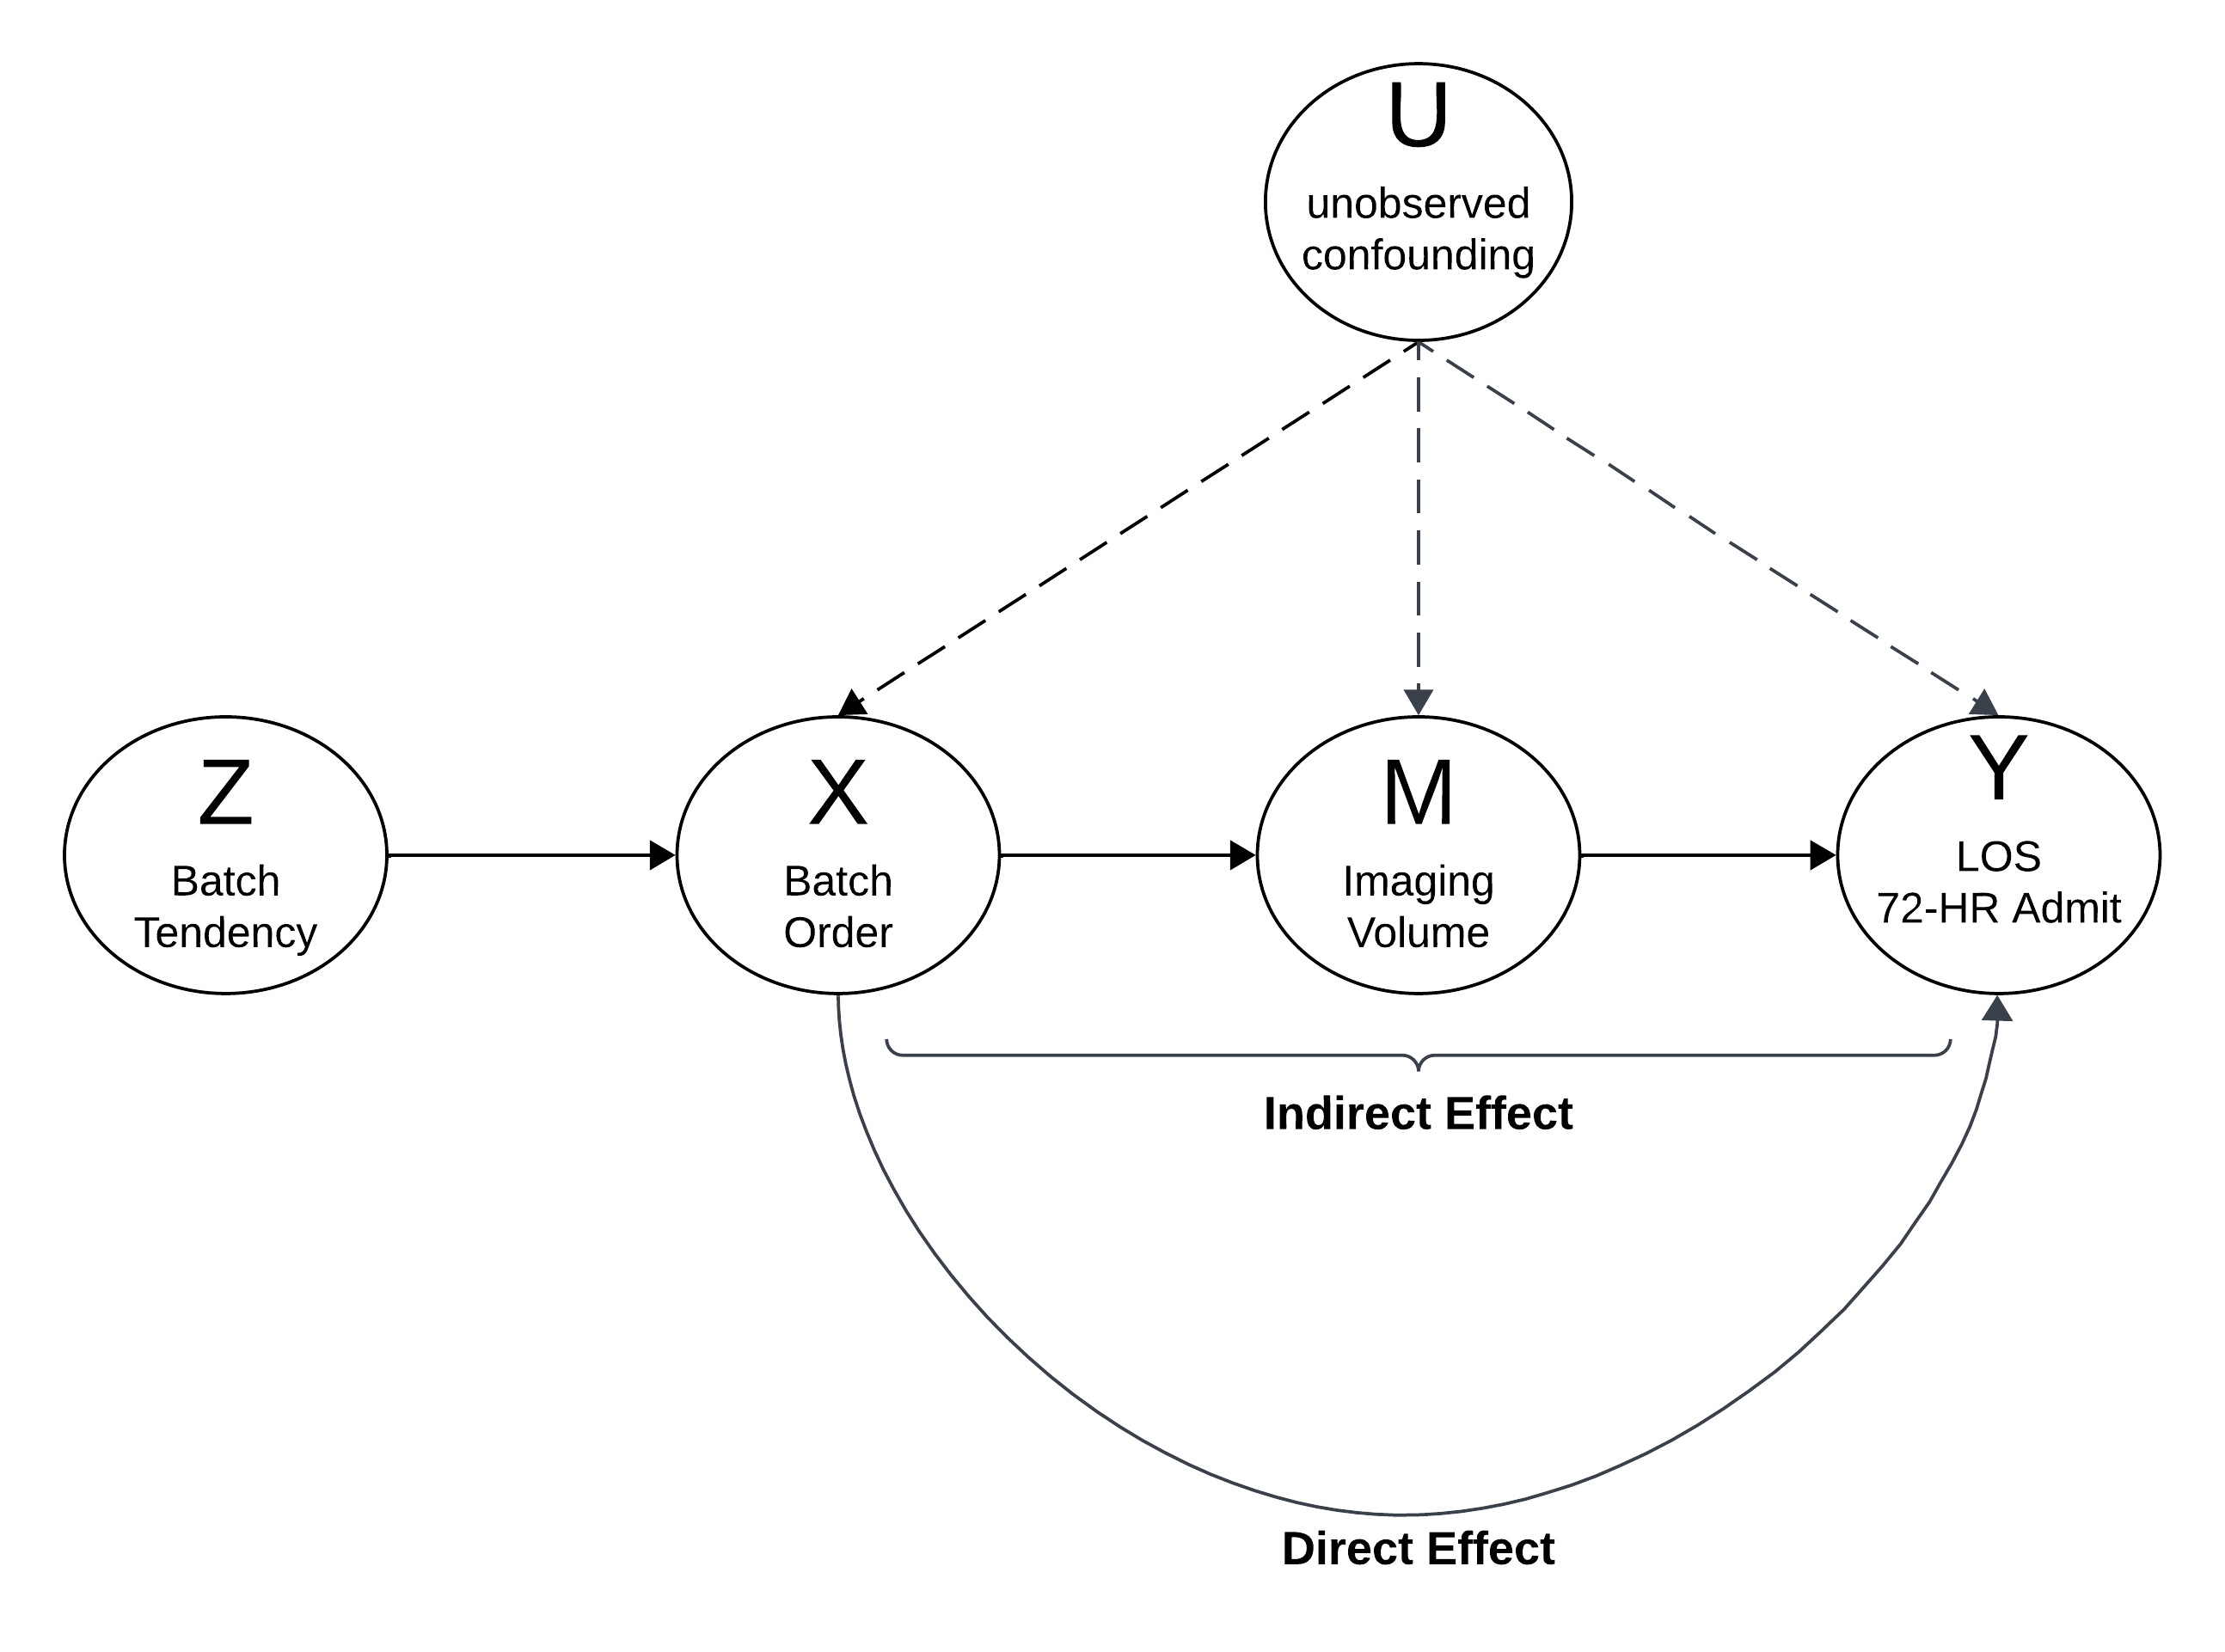
\includegraphics[width=3in]{model.png}
\caption{Directed Acyclic Graph Representing the Causal Pathways Between Batch Order, Imaging Volume, and ED Outcomes}
\label{fig:dag}
\end{figure}

In this DAG, batch tendency (Z) is used as an instrumental variable to
predict batch order (X), which in turn affects both imaging volume (M)
and our primary outcomes, including ED length of stay and 72-hour return
with admission (Y). The unobserved confounding (U) is assumed to
influence both imaging volume and the outcomes directly. The mediation
analysis supports this structure, as it confirms that imaging volume
mediates the relationship between batch ordering and ED outcomes, albeit
modestly. By identifying this framework through our analysis, we provide
a data-driven explanation for how batching influences ED operations.

\textbf{Interpretation of Mediation Results.}---These results show that
the number of imaging tests serves as a partial mediator in the
relationship between batching and ED outcomes. For length of stay,
increased testing tends to prolong ED visits, but the overall effect of
batching on LOS is negligible. For return visits, the increase in
diagnostic testing slightly reduces the likelihood of a return within 72
hours, though the overall effect remains small and insignificant. These
findings highlight the trade-offs involved in batching diagnostic
orders: while batching may streamline certain processes, the associated
increase in testing has modest effects on patient flow and outcomes.

\newpage

\hypertarget{references}{%
\section*{References}\label{references}}
\addcontentsline{toc}{section}{References}

\hypertarget{refs}{}
\begin{CSLReferences}{1}{0}
\leavevmode\vadjust pre{\hypertarget{ref-akhlaghpour2020value}{}}%
Akhlaghpour, Hessameddin. 2020. {``The Value of Information in
Sequential Decision Making.''} \emph{Proceedings of the National Academy
of Sciences} 117 (48): 30925--31.

\leavevmode\vadjust pre{\hypertarget{ref-armony2015heterogeneous}{}}%
Armony, Mor, Shlomo Israelit, Avishai Mandelbaum, Yariv N Marmor, Yulia
Tseytlin, and Galit B Yom-Tov. 2015. {``On Patient Flow in Hospitals: A
Data-Based Queueing-Science Perspective.''} \emph{Stochastic Systems} 5
(1): 146--94.

\leavevmode\vadjust pre{\hypertarget{ref-asplin2003model}{}}%
Asplin, Brent R, David J Magid, Karin V Rhodes, Leif I Solberg, Nicole
Lurie, and Carlos A Camargo Jr. 2003. {``A Conceptual Model of Emergency
Department Crowding.''} \emph{Annals of Emergency Medicine} 42 (2):
173--80.

\leavevmode\vadjust pre{\hypertarget{ref-naseim2015}{}}%
Balogh, EP, BT Miller, and JR Ball. 2015. \emph{Improving Diagnosis in
Health Care}. Edited by Committee on Diagnostic Error in Health Care,
Board on Health Care Services, Institute of Medicine, The National
Academies of Sciences Engineering, and Medicine. Washington (DC):
National Academies Press (US).

\leavevmode\vadjust pre{\hypertarget{ref-batt2019impact}{}}%
Batt, Robert J, and Christian Terwiesch. 2019. {``The Impact of Process
Design on ED Performance: A Discreteevent Simulation Study.''}
\emph{Production and Operations Management} 28 (6): 1493--1510.

\leavevmode\vadjust pre{\hypertarget{ref-bernstein2009}{}}%
Bernstein, SL, D Aronsky, R Duseja, S Epstein, D Handel, U Hwang, M
McCarthy, et al. 2009. {``The Effect of Emergency Department Crowding on
Clinically Oriented Outcomes.''} \emph{Academic Emergency Medicine} 16
(1): 1--10.

\leavevmode\vadjust pre{\hypertarget{ref-bernstein2009effect}{}}%
Bernstein, Steven L, Dominik Aronsky, Reena Duseja, Stephen Epstein, Dan
Handel, Ula Hwang, Melissa McCarthy, et al. 2009. {``The Effect of
Emergency Department Crowding on Clinically Oriented Outcomes.''}
\emph{Academic Emergency Medicine} 16 (1): 1--10.

\leavevmode\vadjust pre{\hypertarget{ref-bhuller2020incarceration}{}}%
Bhuller, Manudeep, Gordon B Dahl, Katrine V Løken, and Magne Mogstad.
2020. {``Incarceration, Recidivism, and Employment.''} \emph{Journal of
Political Economy} 128 (4): 1269--1324.

\leavevmode\vadjust pre{\hypertarget{ref-cooke2013overview}{}}%
Cooke, Georga, Amanda Tapley, Elizabeth Holliday, Simon Morgan, Kim
Henderson, Jean Ball, Mieke van Driel, Neil Spike, Rohan Kerr, and
Parker Magin. 2013. {``An Overview of Clinical Decision Making: Biases
and Guidelines.''} \emph{BMJ} 346: f1239.

\leavevmode\vadjust pre{\hypertarget{ref-croskerry2013cognitive}{}}%
Croskerry, Pat. 2013. {``From Mindless to Mindful Practice---Cognitive
Bias and Clinical Decision Making.''} \emph{New England Journal of
Medicine} 368 (26): 2445--48.

\leavevmode\vadjust pre{\hypertarget{ref-dai2010load}{}}%
Dai, Jim, and Shuangchi He. 2010. {``Load Balancing and Capacity
Planning in Queueing Networks with Abandonment.''} \emph{Operations
Research} 58 (2): 429--39.

\leavevmode\vadjust pre{\hypertarget{ref-dixit1994investment}{}}%
Dixit, Avinash K, and Robert S Pindyck. 1994. \emph{Investment Under
Uncertainty}. Princeton university press.

\leavevmode\vadjust pre{\hypertarget{ref-dobbie2018effects}{}}%
Dobbie, Will, Jacob Goldin, and Crystal S. Yang. 2018. {``The Effects of
Pretrial Detention on Conviction, Future Crime, and Employment: Evidence
from Randomly Assigned Judges.''} \emph{American Economic Review} 108
(2): 201--40.

\leavevmode\vadjust pre{\hypertarget{ref-doyle2015measuring}{}}%
Doyle, Joseph, John Graves, Jonathan Gruber, and Samuel Kleiner. 2015.
{``Measuring Returns to Hospital Care: Evidence from Ambulance Referral
Patterns.''} \emph{Journal of Political Economy} 123 (1): 170--214.
\url{https://doi.org/10.1086/677756}.

\leavevmode\vadjust pre{\hypertarget{ref-eichmeyer2022pathways}{}}%
Eichmeyer, Sarah, and Jonathan Zhang. 2022. {``Pathways into Opioid
Dependence: Evidence from Practice Variation in Emergency
Departments.''} \emph{American Economic Journal: Applied Economics} 14
(4): 271--300. \url{https://doi.org/10.1257/app.20210048}.

\leavevmode\vadjust pre{\hypertarget{ref-forster2003effect}{}}%
Forster, Alan J, Ian Stiell, George Wells, Alexander J Lee, and Carl Van
Walraven. 2003. {``The Effect of Hospital Occupancy on Emergency
Department Length of Stay and Patient Disposition.''} \emph{Academic
Emergency Medicine} 10 (2): 127--33.

\leavevmode\vadjust pre{\hypertarget{ref-garg2018value}{}}%
Garg, Ashish, Yingjie Wang, and Ricardo Valerdi. 2018. {``The Value of
Options in Emergency Response Management.''} \emph{Systems Engineering}
21 (4): 344--59.

\leavevmode\vadjust pre{\hypertarget{ref-green2006managing}{}}%
Green, Linda V. 2006. {``Managing Patient Demand in Healthcare
Systems.''} \emph{Encyclopedia of Health Economics} 2: 33--39.

\leavevmode\vadjust pre{\hypertarget{ref-jarvis2016ed}{}}%
Jarvis, Paul RK. 2016. {``ED Overcrowding and the Full Capacity Protocol
Cross over Study: What Happens When a Hospital Is over Capacity?''}
\emph{Emergency Medicine Journal} 33 (2): 115--23.

\leavevmode\vadjust pre{\hypertarget{ref-johnson2019decision}{}}%
Johnson, Gordon. 2019. {``Decision Making in Emergency Medicine:
Rational, Improvisational or Both?''} \emph{Emergency Medicine
Australasia} 31 (4): 525--26.

\leavevmode\vadjust pre{\hypertarget{ref-kanzaria2015emergency}{}}%
Kanzaria, Hemal K, Jerome R Hoffman, Marc A Probst, John P Caloyeras,
Sandra H Berry, and Robert H Brook. 2015. {``Emergency Physician
Perceptions of Medically Unnecessary Advanced Diagnostic Imaging.''}
\emph{Academic Emergency Medicine} 22 (4): 390--98.

\leavevmode\vadjust pre{\hypertarget{ref-koch2018}{}}%
Koch, C, K Roberts, C Petruccelli, and DJ Morgan. 2018. {``The Frequency
of Unnecessary Testing in Hospitalized Patients.''} \emph{Am J Med} 131
(5): 500--503. \url{https://doi.org/10.1016/j.amjmed.2017.11.025}.

\leavevmode\vadjust pre{\hypertarget{ref-kocher2012effect}{}}%
Kocher, Keith E, William J Meurer, Jeffrey S Desmond, and Brahmajee K
Nallamothu. 2012. {``Effect of Testing and Treatment on Emergency
Department Length of Stay Using a National Database.''} \emph{Academic
Emergency Medicine} 19 (5): 525--34.

\leavevmode\vadjust pre{\hypertarget{ref-morley2018emergency}{}}%
Morley, Claire, Maria Unwin, Gregory M Peterson, Jim Stankovich, and
Leigh Kinsman. 2018. {``Emergency Department Crowding: A Systematic
Review of Causes, Consequences and Solutions.''} \emph{PloS One} 13 (8):
e0203316.

\leavevmode\vadjust pre{\hypertarget{ref-nibbelink2018emergency}{}}%
Nibbelink, Christine W, and Barbara B Brewer. 2018. {``Emergency Nursing
Decision Making: Experience, Expertise, and Cognitive Strategies.''}
\emph{Journal of Emergency Nursing} 44 (4): 360--68.

\leavevmode\vadjust pre{\hypertarget{ref-o2018overdiagnosis}{}}%
O'Connor, Raymond E, and Graham Nichol. 2018. {``Overdiagnosis and
Overtreatment: Generalists---It's Time for a Grassroots Revolution.''}
\emph{BMJ} 362: k2820.

\leavevmode\vadjust pre{\hypertarget{ref-pines2010national}{}}%
Pines, Jesse M, Peter M Mullins, Joshua K Cooper, Lisa B Feng, and Karin
E Roth. 2010. {``National Trends in Emergency Department Use, Care
Patterns, and Quality of Care of Older Adults in the United States.''}
\emph{Journal of the American Geriatrics Society} 58 (12): 2281--87.

\leavevmode\vadjust pre{\hypertarget{ref-rosen2018quality}{}}%
Rosen, Charlotte L, and Gilbert Seda. 2018. {``Quality Improvement in
Acute Care: How to Improve Your Emergency Department Right Now.''}
\emph{Emergency Medicine Clinics} 36 (4): 835--51.

\leavevmode\vadjust pre{\hypertarget{ref-sabbatini2016overzealous}{}}%
Sabbatini, Amber K, Luciano M Prevedello, Ali S Raja, Michael F Fialkow,
Aaron D Sodickson, and Ramin Khorasani. 2016. {``Overzealous Use of the
CT Scanner: How an ED Medical Director Can Use Data to Change Physician
Behavior.''} \emph{Emergency Radiology} 23 (2): 173--79.

\leavevmode\vadjust pre{\hypertarget{ref-saghafian2015}{}}%
Saghafian, S, G Austin, and SJ Traub. 2015. {``Operations
Research/Management Contributions to Emergency Department Patient Flow
Optimization: Review and Research Prospects.''} \emph{IIE Transactions
on Healthcare Systems Engineering} 5 (2): 101--23.

\leavevmode\vadjust pre{\hypertarget{ref-shi2016models}{}}%
Shi, Pengyi, Mabel C Chou, Jim G Dai, Dingfan Ding, and Jing Sim. 2016.
{``Models and Insights for Hospital Inpatient Operations: Time-Dependent
ED Boarding Time.''} \emph{Management Science} 62 (1): 1--28.

\leavevmode\vadjust pre{\hypertarget{ref-smith2013impact}{}}%
Smith, Michael, Craig Feied, Jonathan Handler, Michael Gillam, and
William Chunn. 2013. {``The Impact of Using Emergency Physicians in the
ED.''} \emph{The American Journal of Emergency Medicine} 31 (1):
154--60.

\leavevmode\vadjust pre{\hypertarget{ref-song2020managing}{}}%
Song, Hummy, Anita L Tucker, Rachel Graue, Sarah Moravick, and Jillian J
Yang. 2020. {``Managing Hospital Inpatient Bed Capacity Through
Partitioning Care into Focused Wings.''} \emph{Manufacturing \& Service
Operations Management} 22 (1): 70--87.

\leavevmode\vadjust pre{\hypertarget{ref-studdert2005defensive}{}}%
Studdert, David M, Michelle M Mello, William M Sage, Catherine M
DesRoches, Jordon Peugh, Kinga Zapert, and Troyen A Brennan. 2005.
{``Defensive Medicine Among High-Risk Specialist Physicians in a
Volatile Malpractice Environment.''} \emph{Jama} 293 (21): 2609--17.

\leavevmode\vadjust pre{\hypertarget{ref-traub2016emergency}{}}%
Traub, Stephen J, Cameron F Stewart, Reza Didehban, Adam C Bartley,
Soroush Saghafian, Vernon D Smith, Scott M Silvers, Ryan LeCheminant,
and Christopher A Lipinski. 2016. {``Emergency Department Rotational
Patient Assignment.''} \emph{Annals of Emergency Medicine} 67 (2):
206--15. \url{https://doi.org/10.1016/j.annemergmed.2015.07.008}.

\leavevmode\vadjust pre{\hypertarget{ref-wang2019data}{}}%
Wang, Jingui, Yanfeng Ouyang, Xiaobo Qu, and Jingshan Li. 2019.
{``Data-Driven Patient Scheduling in Emergency Departments: A Hybrid
Robust-Stochastic Approach.''} \emph{Flexible Services and Manufacturing
Journal} 31 (4): 1174--1202.

\leavevmode\vadjust pre{\hypertarget{ref-welch2011overdiagnosed}{}}%
Welch, H Gilbert, Lisa Schwartz, and Steve Woloshin. 2011.
\emph{Overdiagnosed: Making People Sick in the Pursuit of Health}.
Beacon Press.

\leavevmode\vadjust pre{\hypertarget{ref-zychlinski2019discrete}{}}%
Zychlinski, Natalia, Avishai Mandelbaum, Petar Momcilovic, and Izack
Cohen. 2019. {``A Discrete-Event Simulation Model for Managing Urgent
Care Units.''} \emph{Operations Research for Health Care} 23: 100202.

\end{CSLReferences}

\bibliographystyle{unsrt}
\bibliography{references.bib}


\end{document}
